\documentclass[12pt]{article}
\usepackage[paper=letterpaper,margin=2cm]{geometry}

\usepackage {mathtools, amssymb, amsthm}
\usepackage{graphicx}
\usepackage{tabularx}
\usepackage{titling}
\usepackage{float}
\usepackage{enumerate}
%%\usepackage[table,xcdraw]{xcolor}
\usepackage{fancyhdr}
\usepackage{polynom}
\usepackage{caption, booktabs}
\usepackage{makecell}
%%\usepackage{cellspace}
%%\setlength\cellspacetoplimit{5pt}
%%\setlength\cellspacebottomlimit{5pt}
	
\pagestyle{fancy}
\fancyhf{}
\rhead{\small {© 2022 All Rights Reserved, Aiden Rosenberg}}
\rfoot{Page \thepage}

\setlength{\droptitle}{-6em}

\title{AP Classroom Problems}
\author{Aiden Rosenberg}
\date{2022 - 2023 A.D}
\begin{document}



\maketitle
\section*{2.01}
\begin{enumerate}
    \item If $P(t)$ is the size of a population at time t, which of the following differential equations describes linear growth in the size of the population?
   $$ \boxed{\frac{dP}{dt}=200}$$
    \item 
   
    \begin{center}
        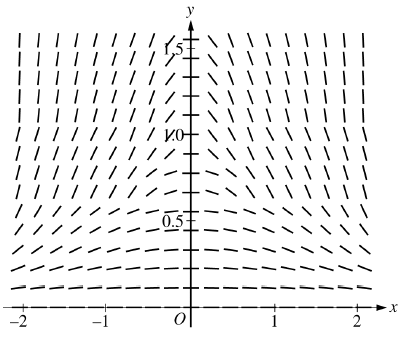
\includegraphics[scale=0.75]{original.png}
    \end{center}
    The slope field for a certain differential equation is shown above. Which of the following could be a solution to the differential equation with the initial condition $y(0)=1$?
    $$\boxed{y=\frac{1}{1+x^2}}$$
    \item 
     \begin{center}
        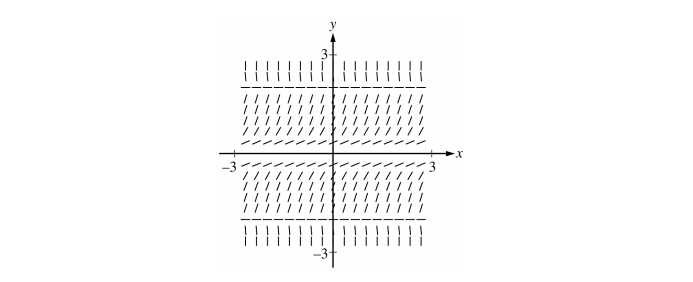
\includegraphics[scale=1]{original-1.png}
    \end{center}
    Shown above is a slope field for the differential equation $\frac{dy}{dx}=y^2(4-y^2)$. If $y = g(x)$ is the solution to the differential equation with the initial condition $g(-2)=-1$, then, $\lim_{x\to\infty} g(x)$ is
    $$\boxed{\lim_{x\to\infty} g(x)=0}$$
    \item For what value of $k$, if any, is $y=e^{2x}+ke^{-3x}$ a solution to the differential equation $4y-y''=10e^{-3x}$ ?
    \begin{enumerate}
        \item $\frac{dy}{dx}=2e^{2x}-3ke^{-3x}$
        \item $\frac{d^2y}{dx^2}=4e^{2x}+9ke^{-3x}$
    \end{enumerate}
    $$4(e^{2x}+ke^{-3x})-(4e^{2x}+9ke^{-3x})=10e^{3x}$$
    $$4e^{2x}+4ke^{-3x}-4e^{2x}-9ke^{-3x}=10e^{3x}$$
    $$4ke^{-3x}-9ke^{-3x}=10e^{3x}$$
    $$-5ke^{-3x}=10e^{3x}$$
    
   $$ \boxed{\therefore k=-2}$$
   \item Of the following, which are solutions to the differential equation $y''-10y'+9y=0$
   \begin{enumerate} [i.]
       \item $y=2\sin(3x)$
       $$\frac{dy}{dx}=6\cos(3x) \Longrightarrow \frac{d^2y}{dx^2}=-18\sin(3x)$$
       $$-18\sin(3x)-60\cos(3x)+18\sin(3x)\neq 0$$
       \item $y=5e^x$
        $$\frac{dy}{dx}=5e^x \Longrightarrow \frac{d^2y}{dx^2}=5e^x$$
        $$5e^x-50e^x+45e^x=0$$
       \item $y=Ce^{9x}$, where $C$ is a constant.
        $$\frac{dy}{dx}=Ce^{9x} \Longrightarrow \frac{d^2y}{dx^2}=Ce^{9x}$$
         $$Ce^{9x}-10e^{9x}+45Ce^{9x}=0$$
   \end{enumerate}
\boxed{\text{II and III only}}

\item 
\begin{center}
        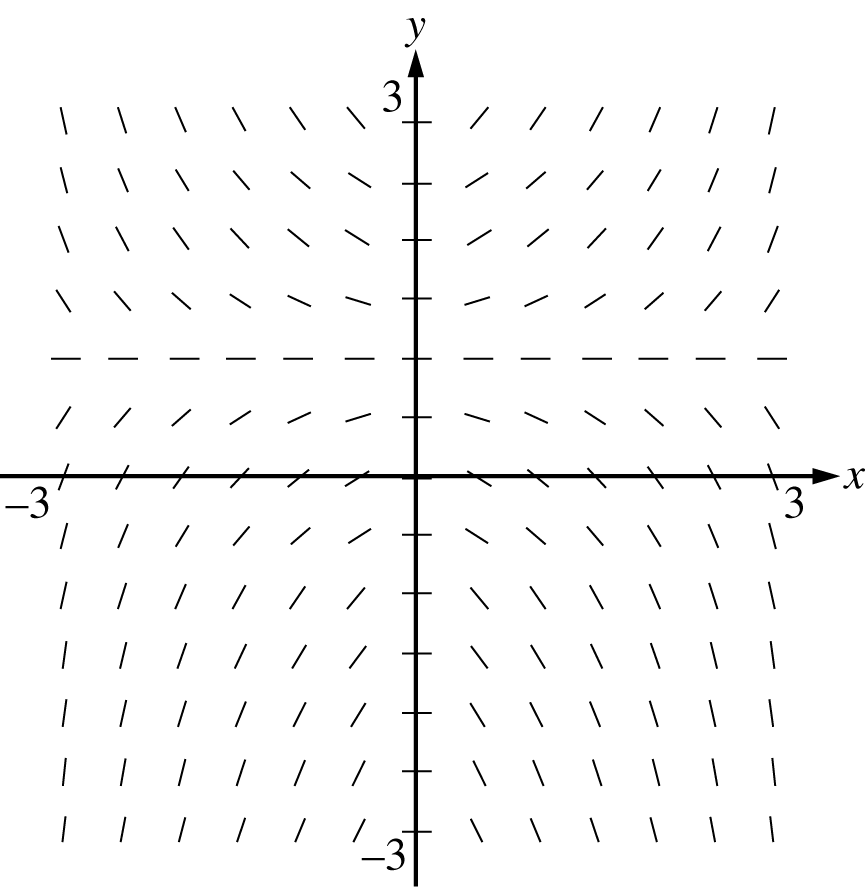
\includegraphics[scale=1]{original-2.png}
    \end{center}
Shown above is a slope field for which of the following differential equations?
$$\boxed{\frac{dy}{dx}=xy-x}$$

\item Which of the following is a slope field for the differential equation $\frac{dy}{dx}=\frac{x}{y}$?
\begin{center}
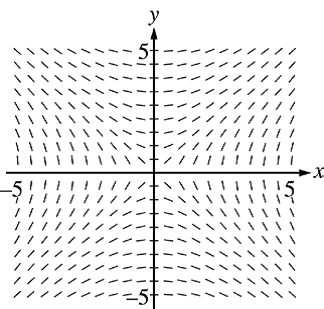
\includegraphics[]{original-3.png}
\end{center}

\item 
\begin{center}
    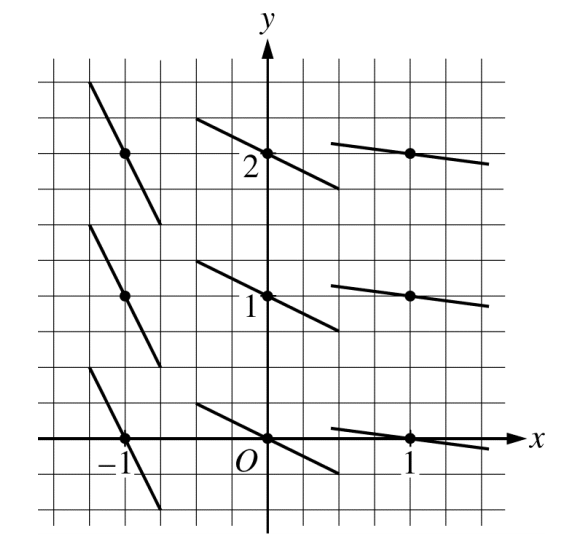
\includegraphics[scale=0.5]{original-4.png}
\end{center}

A slope field for a differential equation is shown in the figure above. If $y = f(x)$ is the particular solution to the differential equation through the point $(-1,2)$ and $h(x) = 3x\cdot f(x)$, then $h'(-1) =$
$$h'(x)=3\cdot f(x) + 3x\cdot f'(x)$$
$$h'(-1)=3\cdot f(-1) + 3(-1)\cdot f'(-1)$$
$$h'(-1)=6 -3\cdot (-2)$$
$$h'(-1)=6 -3\cdot (-2)$$
$$\boxed{h'(-1)=12}$$

\item The rate of change of the volume, $V$, of water in a tank with respect to time, $t$, is directly proportional to the square root of the volume. Which of the following is a differential equation that describes this relationship?
$$\boxed{\frac{dV}{dt}=k \sqrt{V}}$$

\item The rate at which a quantity $M$ of a certain radioactive substance decays is proportional to the amount of the substance present at a given time. Which of the following is a differential equation that could describe this relationship?
$$\boxed{\frac{dM}{dt}=-0.11M}$$
\end{enumerate}

\section*{2.02}
\begin{enumerate}
    \item Let $y=f(x)$ be the solution to the differential equation $\frac{dy}{dx}=2x+y$ with initial condition $f(1)=0$. What is the approximation for $f(2)$ obtained by using Euler’s method with two steps of equal length, starting at $x=1$

\begin{table}[H]
\caption{$\Delta x = 0.5$}
\centering \label{table_example}
\begin{tabular}{l|lll}
$x$ & \multicolumn{1}{l|}{$y$} & \multicolumn{1}{l|}{$\frac{dy}{dx}$} & $\Delta y$ \\ \hline
1 & 0 & 2 & 1 \\
1.5 & 1 & 4 & 2 \\
2 & 3 &  & 
\end{tabular}
\end{table}
$$\boxed{f(2) \approx 3.0}$$

\item Let $y=f(x)$ be the solution to the differential equation $\frac{dy}{dx}=x-y$ with initial condition $f(1)=3$. What is the approximation for $f(2)$ obtained by using Euler’s method with two steps of equal length starting at $x=1$?

\begin{table}[H]
\caption{$\Delta x = 0.5$}
\centering \label{table_example}
\begin{tabular}{l|lll}
$x$ & \multicolumn{1}{l|}{$y$} & \multicolumn{1}{l|}{$\frac{dy}{dx}$} & $\Delta y$ \\ \hline
1 & 3 & -2 & -1 \\
1.5 & 2 & -0.5 & -0.25 \\
2 & 1.75 &  & 
\end{tabular}
\end{table}
$$\boxed{f(2) \approx 1.75}$$
    
    \item 
\begin{table}[H]
\centering
\begin{tabular}{l|lll}
$x$     & 1   & 1.5 & 2   \\ \hline
$f'(x)$ & 0.2 & 0.5 & 0.9
\end{tabular}
\end{table}
The table above gives values of $f'$, the derivative of a function $f$. If $f(1)=4$, what is the approximation to $f(2)$ obtained by using Euler’s method with a step size of $0.5$ ?

\begin{table}[H]
\caption{$\Delta x = 0.5$}
\centering \label{table_example}
\begin{tabular}{l|lll}
$x$ & \multicolumn{1}{l|}{$y$} & \multicolumn{1}{l|}{$\frac{dy}{dx}$} & $\Delta y$ \\ \hline
1 & 4 & 0.2 & 0.1 \\
1.5 & 4.1 & 0.5 & 0.25 \\
2 & 4.35 &  & 
\end{tabular}
\end{table}
$$\boxed{f(2)\approx 4.35}$$

\item Given that $y(1) =-3$ and $\frac{dy}{dx}=2x+y$, what is the approximation for $y(2)$ if Euler’s method is used with a step size of $0.5$, starting at $x = 1$ ?

\begin{table}[H]
\caption{$\Delta x = 0.5$}
\centering \label{table_example}
\begin{tabular}{l|lll}
$x$ & \multicolumn{1}{l|}{$y$} & \multicolumn{1}{l|}{$\frac{dy}{dx}$} & $\Delta y$ \\ \hline
1 & -3 & -1 & -0.5 \\
1.5 & -3.5 & -0.5 & -0.25 \\
2 & -3.75 &  & 
\end{tabular}
\end{table}
$$\boxed{y(2) \approx -3.75}$$


\item 
\begin{table}[H]
\centering
\begin{tabular}{l|lllllll}
$x$     & -1.0 & -0.5 & 0.0 & 0.5 & 1.0 & 1.5 & 2.0 \\ \hline
$g'(x)$ & 2    & 4    & 3   & 1   & 0   & -3  & -6 
\end{tabular}
\end{table}

The table above gives selected values for the derivative of a function $g$ on the interval \\ $ -1 \leq x \leq 2$. If $g(-1) = -2$ and Euler’s method with a step-size of $1.5$ is used to approximate $g(2)$, what is the resulting approximation?

\begin{table}[H]
\caption{$\Delta x = 1.5$}
\centering \label{table_example}
\begin{tabular}{l|lll}
$x$ & \multicolumn{1}{l|}{$y$} & \multicolumn{1}{l|}{$\frac{dy}{dx}$} & $\Delta y$ \\ \hline
-1 & -2 & 2 & 3 \\
0.5 & 1 & 1 & 1.5 \\
2 & 2.5 &  & 
\end{tabular}
\end{table}
$$\boxed{g(2) \approx 2.5}$$

\item 
\begin{table}[h!]
\centering
\begin{tabular}{l|lll}
$x$     & 2    & 2.2  & 2.4  \\ \hline
$f'(x)$ & -0.5 & -0.3 & -0.1
\end{tabular}
\end{table}
Let $y = f(x)$ be the solution to the differential equation $\frac{dy}{dx}=f'(x$) with initial condition $f(2) = 3$. Selected values of $f'$ are given in the table above. What is the approximation for $f(2.4)$ if Euler’s method is used, starting at $x = 2$ with two steps of equal size?
\begin{table}[H]
\caption{$\Delta x = 0.2$}
\centering \label{table_example}
\begin{tabular}{l|lll}
$x$ & \multicolumn{1}{l|}{$y$} & \multicolumn{1}{l|}{$\frac{dy}{dx}$} & $\Delta y$ \\ \hline
2 & 3 & -0.5 & -0.1 \\
2.2 & 2.9 & -0.3 & -0.06 \\
2.4 & 2.84 &  & 
\end{tabular}
\end{table}
$$\boxed{f(2.4)\approx 2.84}$$

\item Let $y=f(x)$ be the solution to the differential equation $\frac{dy}{dx}=y-10x^2$ with the initial condition $f(0)=3$. What is the approximation for $f(0.4)$ if Euler’s method is used, starting at $x=0$ with steps of size $0.2$?

\begin{table}[H]
\caption{$\Delta x = 0.2$}
\centering \label{table_example}
\begin{tabular}{l|lll}
$x$ & \multicolumn{1}{l|}{$y$} & \multicolumn{1}{l|}{$\frac{dy}{dx}$} & $\Delta y$ \\ \hline
0 & 3 & 3 & 0.6 \\
0.2 & 3.6 & 3.2 & 0.64 \\
0.4 & 4.24 &  & 
\end{tabular}
\end{table}
$$\boxed{f(0.4)\approx 4.24}$$

\item Let $y=g(x)$ be the solution to the differential equation $\frac{dy}{dx}=xy-2$ with the initial condition $g(2)=-1$. What is the approximation for $g(1)$ if Euler’s method is used, starting at $x=2$ with two steps of equal size?
\begin{table}[H]
\caption{$\Delta x = -0.5$}
\centering \label{table_example}
\begin{tabular}{l|lll}
$x$ & \multicolumn{1}{l|}{$y$} & \multicolumn{1}{l|}{$\frac{dy}{dx}$} & $\Delta y$ \\ \hline
2 & -1 & -4 & 2 \\
1.5 & 1 & -0.5 & 0.25 \\
1 & 1.25 &  & 
\end{tabular}
\end{table}
$$\boxed{g(1)\approx 1.25}$$


\item If the pressure $P$ applied to a gas is increased while the gas is held at a constant temperature, then the volume $V $of the gas will decrease. The rate of change of the volume of gas with respect to the pressure is proportional to the reciprocal of the square of the pressure. Which of the following is a differential equation that could describe this relationship?

$$\boxed{\frac{dV}{dP} =\frac{k}{P^2}, \text{ where } k \text{ is a negative constant.}}$$

\item A jogger runs along a straight track. The jogger’s position is given by the function $p(t)$, where $t$ is measured in minutes since the start of the run. During the first minute of the run, the jogger’s acceleration is proportional to the square root of the time since the start of the run. Which of the following is a differential equation that describes this relationship, where k is a positive constant?

$$\boxed{\frac{d^2p}{dt^2}=k \sqrt{t}}$$

\end{enumerate}


\section*{2.03}
\begin{enumerate}
    \item If $\frac{dy}{dx}=4y$ and if $y=4$ when $x=0$, then $y=$
$$\int \frac{dy}{y} = \int 4 \, dx$$
$$\ln|y|=4x+C \biggr\rvert_{(0,4)} \Longrightarrow \ln|4|=C$$ 
$$\ln|y|=4x+\ln(4)$$ 
$$y=4e^{4x}$$ 

    \item Let $y=f(x)$ be the solution to the differential equation $\frac{dy}{dx}=x+y$ with the initial condition $f(1)=2$. What is the approximation for $f(2)$ if Euler’s method is used, starting at $x=1$ with a step size of $0.5$?
\begin{table}[H]
\caption{$\Delta x = 0.5$}
\centering \label{table_example}
\begin{tabular}{l|lll}
$x$ & \multicolumn{1}{l|}{$y$} & \multicolumn{1}{l|}{$\frac{dy}{dx}$} & $\Delta y$ \\ \hline
1 & 2 & 3 & 3.5 \\
1.5 & 3.5 & 5 & 2.5 \\
2 & 6 &  & 
\end{tabular}
\end{table}
$$\boxed{f(2) \approx 6.0}$$

    \item Let $y=f(x)$ be the solution to the differential equation$\frac{dy}{dx}=x-y-1$ with the initial condition $f(1)=-2$ . What is the approximation for $f(1.4)$ if Euler’s method is used, starting at $x=1$ with two steps of equal size?

\begin{table}[H]
\caption{$\Delta x = 0.2$}
\centering \label{table_example}
\begin{tabular}{l|lll}
$x$ & \multicolumn{1}{l|}{$y$} & \multicolumn{1}{l|}{$\frac{dy}{dx}$} & $\Delta y$ \\ \hline
1 & -2 & 2 & 0.4 \\
1.2 & -1.6 & 1.8 & 0.36 \\
1.4 & -1.24 &  & 
\end{tabular}
\end{table}
$$\boxed{f(1.4) \approx -1.24}$$

    \item 

\begin{table}[H]
\centering
\begin{tabular}{l|llll}
$x$     & -0.2 & 0   & 0.2 & 0.4 \\ \hline
$f'(x)$ & 0.8  & 1.2 & 1.7 & 2.3
\end{tabular}
\end{table}

The table above shows values of $f'$, the derivative of a function $f$, for selected values of $x$. If $f(-0.2)=1$, what is the approximation for $f(0.4)$ obtained by using Euler’s method with a step size of 0.2 starting at $x=-0.2$

\begin{table}[H]
\caption{$\Delta x = 0.2$}
\centering \label{table_example}
\begin{tabular}{l|lll}
$x$ & \multicolumn{1}{l|}{$y$} & \multicolumn{1}{l|}{$\frac{dy}{dx}$} & $\Delta y$ \\ \hline
-0.2 & 1 & 0.8 & 0.16 \\
0 & 1.16 & 1.2 & 0.24 \\
0.2 & 1.4 & 1.7 & 0.34 \\
0.4 & 1.74 &  & 
\end{tabular}
\end{table}
$$\boxed{f(0.4) \approx 1.74}$$
\newpage
\item Which of the following is the solution to the differential equation $\frac{dy}{dx}=y^2-(xy)^2$ with the initial condition $y(3)=1$?
\begin{equation*} 
\begin{split}
\frac{dy}{dx} & = y^2-(xy)^2 \\
 & = y^2-y^2x^2\\
 & = y^2(1-x^2)
\end{split}
\end{equation*}
$$\int \frac{1}{y^2}\, dy = \int (1-x^2) \, dx$$
$$\Longrightarrow \frac{-1}{y}=x-\frac{x^3}{3} +C \biggr\rvert_{(3,1)} \Longrightarrow C=5 $$
$$\frac{-3}{y}=3x-x^3 +15 $$
$$y= \frac{-3}{3x-x^3+15}$$


\item Which of the following is the solution to the differential equation $\frac{dy}{dx}=(x-2)(y-2)$ for $y>2$ with the initial condition $y(4)=5$ ?
$$\int \frac{dy}{(y-2)}=\int {(x-2)} \, dx$$
$$\Longrightarrow \ln|y-2|=\frac{x^2}{2}-2x+C \biggr\rvert_{(4,5)} \Longrightarrow C=\ln(3)$$
$$\Longrightarrow |y-2|=3e^{\frac{x^2}{2}-2x}$$
$$\Longrightarrow y=2+3e^{\frac{x^2}{2}-2x}$$

\item What are all solutions to the differential equation $\frac{dy}{dx}=\frac{1}{x \cdot \ln(2)}$?
$$\int \ln(2) \, dy = \frac{1}{x} \, dx$$
$$\Longrightarrow \ln(2) \cdot y = \ln|x|+C$$
$$\Longrightarrow y = \frac{\ln|x|}{\ln(2)}+C$$

\item Let $y=f(x)$ be the solution to the differential equation $\frac{dy}{dx}=y-10x^2$ with the initial condition f$(0)=3$. What is the approximation for $f(0.4)$ if Euler’s method is used, starting at $x=0$ with steps of size $0.2$ ?

\begin{table}[H]
\caption{$\Delta x = 0.2$}
\centering \label{table_example}
\begin{tabular}{l|lll}
$x$ & \multicolumn{1}{l|}{$y$} & \multicolumn{1}{l|}{$\frac{dy}{dx}$} & $\Delta y$ \\ \hline
0 & 3 & 3 & 0.6 \\
0.2 & 3.6 & 3.2 & 0.64 \\
0.4 & 4.24 &  & 
\end{tabular}
\end{table}
$$\boxed{f(0.4) \approx 4.24}$$

\end{enumerate}

\section*{2.04}
\begin{enumerate}
    \item The function $y = e^{3x}-5x+7$ is a solution to which of the following differential equations?
\begin{enumerate}
    \item $y'=3e^{3x}-5$
    \item $y''=9e^{3x}$
\end{enumerate}
$$9e^{3x}-3(3e^{3x}-5)-15=9e^{3x}-9e^{3x}+15-15)$$
$$\boxed{y''-3y'-15=0}$$
    \item A student attempted to solve the differential equation $\frac{dy}{dx}=xy$ with initial condition $y=2$ when $x=0$. In which step, if any, does an error first appear?
    \begin{align}
\int \frac{1}{y} \, dy= \int x \, dx \\
\ln|y|=\frac{x^2}{2}+C \\
|y| = e^{\frac{x^2}{2}}+C \\
\text{Since $y=2$ when $x=0$,} \Longrightarrow 2=e^0+C \\
y= e^{\frac{x^2}{2}} +1
    \end{align}
    $$\boxed{\text{Step 3}}$$
\item The population $P$ of a city grows according to the differential equation $\frac{dP}{dt}=kP$, where $k$ is a constant and $t$ is measured in years. If the population of the city doubles every 12 years, what is the value of $k$?
\begin{enumerate}
    \item $P(0)=P_0$
    \item $P(12)=2P_0$
\end{enumerate}

$$\Longrightarrow \int \frac{dP}{P} = \int k \, dt$$
$$\Longrightarrow \ln|P|=kt +C$$
$$\Longrightarrow P=Ce^{kt}\biggr\rvert_{(0, P_0)} \Longrightarrow C=P_0$$
$$ P=P_0e^{kt} \biggr\rvert_{(12,2P_0)}$$
$$\Longrightarrow 2P_0=P_0e^{12k} \Longrightarrow 2=e^{12k} $$
$$\boxed{k=\frac{\ln 2}{12} \approx 0.05776}$$

\item If $\frac{dy}{dx} = y\sec^2(x)$ and $y(0)=5$, then $y=$
$$\int \frac{1}{y} \, dy =\int \sec^2(x) \, dx$$
$$\Longrightarrow \ln|y|=\tan(x)+C \biggr\rvert_{(0,5)} \Longrightarrow C=\ln(5) $$
$$\ln|y|=\tan(x)+\ln(5)$$
$$y=5e^{\tan x}$$

\item 
\begin{center}
    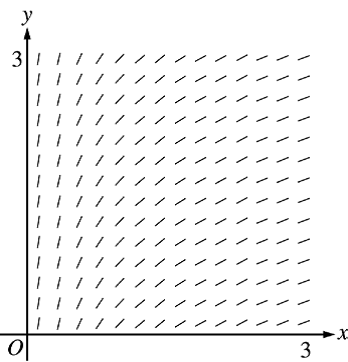
\includegraphics[scale=0.75]{original-5.png}
\end{center}
The slope field for a certain differential equation is shown above. Which of the following could be a specific solution to that differential equation?
$$\boxed{y=\ln(x)}$$

\item The general solution to the differential equation $\frac{dy}{dx}=\frac{x}{y}$ is $y=\pm \sqrt{x^2+C}$ . Let $y=f(x)$ be the particular solution to the differential equation with the initial condition $f(-5)=-4$. Which of the following is an expression for $f(x)$ and its domain?
$$y=\pm \sqrt{x^2+C} \biggr\rvert_{(-5,-4)} \Longrightarrow C=-9$$
$$\boxed{y=-\sqrt{x^2-9} \text{ for } x<-3}$$ 

\item The general solution to the differential equation $\frac{dy}{dx}=\frac{x}{y}$ is $y=\pm \sqrt{x^2+C}$ . Let $y=f(x)$ be the particular solution to the differential equation with the initial condition $f(-2)=-\sqrt{2}$. Which of the following is an expression for $f(x)$ and its domain?
$$y=\pm \sqrt{x^2+C} \biggr\rvert_{(-2,-\sqrt{2})} \Longrightarrow C=-2$$
$$\boxed{y=-\sqrt{x^2-2} \text{ for } x<-\sqrt{2}}$$ 

\item A dose of 400 milligrams of a drug is administered to a patient. The amount of the drug, in milligrams, in the person’s bloodstream at time $t$, in hours, is given by $A(t)$. The rate at which the drug leaves the bloodstream can be modeled by the differential equation $\frac{dA}{dt}=kA$, where k is a constant. Which of the following could be an expression for $A(t)$ ?
$$\ln|A|=kt+C$$
$$\Longrightarrow A=Ce^{kt}$$
$$\boxed{A(t)=400e^{-0.3t}}$$

\item If $y = f(x)$ is a solution to the differential equation $\frac{dy}{dx}=e^{x^2}$ with the initial condition $f(0) = 2$, which of the following is true?
$$y=\int_{0}^{x} e^{t^2} \, dt + C \biggr\rvert_{(0,2)} \Longrightarrow C=2$$
$$\boxed{f(x)=2+\int_{0}^{x} e^{t^2} \, dt}$$
\item Which of the following is the solution to the differential equation $\frac{dy}{dx}=\frac{4x}{y}$ , where $y(2)=-2$?
$$\int y \, dy = \int 4x\,dx$$
$$\frac{y^2}{2}=2x^2+C \biggr\rvert_{(2,-2)} \Longrightarrow C=-6$$
$$\frac{y^2}{2}=2x^2-6 \Longrightarrow y^2=4x^2-12$$
$$y = \pm \sqrt{4x^2-12} \biggr\rvert_{(2,-2)}$$ 
$$\Longrightarrow y=-\sqrt{4x^2-12}$$
$$0=4x^2-12 \Longrightarrow x=\pm \sqrt{3}$$
$$\boxed{y=-\sqrt{4x^2-12} \text{ for } x>\sqrt{3}}$$ 
\end{enumerate}
\section*{2.05}
\begin{enumerate}
    \item A puppy weighs 2.0 pounds at birth and 3.5 pounds two months later. If the weight of the puppy during its first 6 months is increasing at a rate proportional to its weight, then how much will the puppy weigh when it is 3 months old?
    \begin{enumerate}
        \item $W0)=2$ and $W(2)=3.5$
    \end{enumerate}
    $$\Longrightarrow \ln|W|=kt+C \biggr\rvert_{(0,2)} \Longrightarrow C=\ln(2)$$
    $$\Longrightarrow \ln|W|=kt+\ln(2) \Longrightarrow W=2e^{kt}$$
    $$W=2e^{kt} \biggr\rvert_{(2,\frac{7}{2})} \Longrightarrow k=\frac{\ln(\frac{7}{4})}{2}$$
     $$\boxed{W=2e^{t\frac{\ln(\frac{7}{4})}{2}}\biggr\rvert_{(t=3)}\Longrightarrow \frac{7 \cdot \sqrt{7}}{4} \approx 4.630}$$
    
    \item Population $y$ grows according to the equation $\frac{dy}{dx}=ky$ , where is a constant and $t$ is measured in years. If the population doubles every 10 years, then the value of $k$ is?
    begin{enumerate}
\begin{enumerate}
    \item $P(0)=P_0$
    \item $P(10)=2P_0$
\end{enumerate}

$$\Longrightarrow \int \frac{dP}{P} = \int k \, dt$$
$$\Longrightarrow \ln|P|=kt +C$$
$$\Longrightarrow P=Ce^{kt}\biggr\rvert_{(0, P_0)} \Longrightarrow C=P_0$$
$$ P=P_0e^{kt} \biggr\rvert_{(10,2P_0)}$$
$$\Longrightarrow 2P_0=P_0e^{10k} \Longrightarrow 2=e^{10k} $$
$$\boxed{k=\frac{\ln 2}{10} \approx 0.069314}$$

    \item Bacteria in a certain culture increase at a rate proportional to the number present. If the number of bacteria doubles in three hours, in how many hours will the number of bacteria triple?
\begin{enumerate}
    \item $P(0)=P_0$
    \item $P(3)=2P_0$
\end{enumerate}

$$\Longrightarrow \int \frac{dP}{P} = \int k \, dt$$
$$\Longrightarrow \ln|P|=kt +C$$
$$\Longrightarrow P=Ce^{kt}\biggr\rvert_{(0, P_0)} \Longrightarrow C=P_0$$
$$ P=P_0e^{kt} \biggr\rvert_{(3,2P_0)}$$
$$\Longrightarrow 2P_0=P_0e^{3k} \Longrightarrow 2=e^{3k} $$
$$k=\frac{\ln 2}{3}$$
$$P=P_0e^{\frac{\ln 2}{3} \cdot t} \biggr\rvert_{P=3P_0} \Longrightarrow 3=e^{\frac{\ln 2}{3} \cdot t}$$
$$\boxed{\Longrightarrow t=\frac{3\ln(3)}{\ln(2)}}$$
    
    \item During a certain epidemic, the number of people that are infected at any time increases at a rate proportional to the number of people that are infected at that time. If 1,000 people are infected when the epidemic is first discovered, and 1,200 are infected 7 days later, how many people are infected 12 days after the epidemic is first discovered?
\begin{enumerate}
    \item $P(0)=1,000$
    \item $P(7)=1,200$
\end{enumerate}

$$\Longrightarrow \int \frac{dP}{P} = \int k \, dt$$
$$\Longrightarrow \ln|P|=kt +C$$
$$\Longrightarrow P=Ce^{kt}\biggr\rvert_{(0, 1000)} \Longrightarrow C=1000$$
$$ P=1000e^{kt} \biggr\rvert_{(7,1200)}$$
$$\Longrightarrow k=\frac{\ln(1.2)}{7}$$
$$\Longrightarrow P=1000e^{\frac{\ln(1.2)}{7} \cdot t} \biggr\rvert_{t=12}$$
$$\boxed{P(12)=240\cdot 6^{\frac{5}{7}} \cdot 5^{\frac{2}{7}} \approx 1,367}$$
    
    \item Extreme heat applied to a colony of microorganisms causes the size $P$ of the colony, measured in grams, to decrease according to the exponential decay model $\frac{dP}{dt}=-0.4P$, where the time $t$ is measured in hours. The size $Q$ of a second colony of microorganisms, also measured in grams, decreases at the constant rate of 1 gram per hour according to the linear model $\frac{dQ}{dt}=-1$. If at time t=0 the first colony has size $P(0)=2$ and the second colony has size $Q(0)=3$, at what time will both colonies have the same size?

   $$ \ln|P|=0.4t+C \Longrightarrow P(t)=Ce^{-0.4t} \biggr\rvert_{(0,2)} \Longrightarrow C=2$$
    $$Q(t)=C-t \biggr\rvert_{(0,3)} \Longrightarrow C=3$$
$$Q(t)=P(t) \Longleftrightarrow 3-t=2e^{-0.4t}$$
$$\boxed{t \approx 2.156}$$
    
    \item A kitten weighs 85 grams at birth. During the first four weeks after the kitten’s birth, its weight in grams is given by the function $W$ that satisfies the differential equation $\frac{dW}{dt}=kW$, where $t$ is measured in days and $k$ is some positive constant. Which of the following could be an expression for $W(t)$?
    $$W=Ce^{kt}\biggr\rvert_{(0,85)} \Longrightarrow C=85$$ 
    $$\boxed{W(t)=85e^{kt}}$$
    \item During a chemical reaction, the rate of change of the amount of the chemical remaining is proportional to the amount remaining. At time $t=0$, the amount of the chemical is 12 moles. At time $t=4$, the amount of the chemical is 4 moles. At what time $t$ is the amount of the chemical 3 moles? (A mole is a unit of measure used in chemistry.)
    \begin{enumerate}
        \item $A(0)=12$ \& $A(4)=4$
    \end{enumerate}
$$\Longrightarrow \ln|A|=kt +C$$
$$\Longrightarrow A=Ce^{kt}\biggr\rvert_{(0, 12)} \Longrightarrow C=12$$
$$ A=12e^{kt} \biggr\rvert_{(4,4)}$$
$$\Longrightarrow k=\frac{\ln(\frac{1}{3})}{4}$$
$$\Longrightarrow A=12e^{\frac{1}{4} \ln(\frac{1}{3}) \cdot t}$$
$$3=12e^{\frac{1}{4} \ln(\frac{1}{3}) \cdot t} \Longrightarrow t=\frac{4\ln(\frac{1}{4})}{\ln(\frac{1}{3})}$$
$$\boxed{t=\frac{4\ln(4)}{\ln(3)}}$$

    
    \item  A dose of 400 milligrams of a drug is administered to a patient. The amount of the drug, in milligrams, in the person’s bloodstream at time $t$, in hours, is given by $A(t)$. The rate at which the drug leaves the bloodstream can be modeled by the differential equation $\frac{dA}{dt}=kA$, where $k$ is a constant. Which of the following could be an expression for $A(t)$?
    \begin{enumerate}
        \item $A(0)=400$
    \end{enumerate}
    $$A(t)=Ce^{kt} \biggr\rvert_{(0,400)} \Longrightarrow C=400$$
    $$A(t)=400e^{kt}$$
    $$\boxed{A(t)=400e^{-0.3t}}$$
    \item During optimal conditions, the rate of change of the population of a certain organism is proportional to the population at time $t$, in hours. At time $t=0$ hours, the population is 300. At time $t=24$ hours, the population is 1000. At what time $t$ is the population 500?
    \begin{enumerate}
        \item $P(0)=300$
        \item $P(24)=1000$
    \end{enumerate}
$$\Longrightarrow P=Ce^{kt}\biggr\rvert_{(0, 300)} \Longrightarrow C=300$$
$$ P=300e^{kt} \biggr\rvert_{(24,1000)}$$
$$\Longrightarrow k=\frac{\ln(\frac{10}{3})}{24}$$
$$\Longrightarrow P=300e^{\frac{\ln(\frac{10}{3})}{24} \cdot t}$$
$$500=300e^{\frac{\ln(\frac{10}{3})}{24} \cdot t} \Longrightarrow \ln \biggr(\frac{5}{3}\biggr) = \frac{1}{24}\ln\biggr(\frac{10}{3}\biggr) \cdot t$$
$$\boxed{t=\frac{24\ln \biggr(\frac{5}{3}\biggr)}{\ln\biggr(\frac{10}{3}\biggr)}}$$
    
    \item If $\frac{dy}{dt}=ky$ and $k$ is a nonzero constant, then $y(x)$ could be
    $$y(x)=Ce^{kt}$$
    $$\boxed{y(x)=2e^{kt}}$$
\end{enumerate}
\section*{2.06}
\begin{enumerate}
    \item The number of antibodies $y$ in a patient’s bloodstream at time $t$ is increasing according to a logistic differential equation. Which of the following could be the differential equation?
    $$\boxed{\frac{dy}{dx}=0.025y \cdot (5000-y)}$$
    \item The rate of change $\frac{dP}{dt}$ of the number of people on an ocean beach is modeled by a logistic differential equation. The maximum number of people allowed on the beach is 1200. At 10 A.M., the number of people on the beach is 200 and is increasing at the rate of 400 people per hour. Which of the following differential equations describes the situation?
    $$\boxed{\frac{dP}{dt}=\frac{1}{500}P(1200-P)}$$
    \item Let $k$ be a positive constant. Which of the following is a logistic differential equation?
    $$\boxed{\frac{dy}{dt} = ky(1-y)}$$
    \item The rate of change, $\frac{dP}{dt}$, of the number of people entering a movie theater is modeled by a logistic differential equation. The capacity of the theater is 500 people. At a certain time, the number of people in the theater is 100 and is increasing at the rate of 50 per minute. Which of the following differential equations could describe this situation?
       $$\boxed{\frac{dP}{dt}=\frac{1}{800}P(500-P)}$$
    \item The total number of reported cases of an illness in a large city $t$ days after the start of an outbreak is modeled by the function $y=F(t)$ that is a solution to the logistic differential equation $\frac{dy}{dx}=\frac{y}{5600}(1400-y)$. If there are 5 reported cases of the illness initially, what is the limiting value for the total number of reported cases of the illness as $t$ increases?
    $$\boxed{\lim_{t\to\infty} F(t) = 1,400}$$
\end{enumerate}

\section*{2.07}
\begin{enumerate}
    \item A population $y$ changes at a rate modeled by the differential equation $\frac{dy}{dt}=0.2y(1000-y)$, where $t$ is measured in years. What are all values of $y$ for which the population is increasing at a decreasing rate?
    $$\frac{d^2y}{dt^2}=\frac{dy}{dt} \biggr(200-\frac{2y}{5} \biggr)$$
    $$\boxed{y \in (500, 1000) \Longrightarrow \frac{d^2y}{dt^2} < 0 }$$
    \item The size of a bird population is modeled by the function $P$ that is a solution to the logistic differential equation $\frac{dP}{dt}=\frac{P}{3}-\frac{P^2}{2100}$, where $t$ is measured in years for $t\geq 0$ and the initial population satisfies $P(0)>0$. Which of the following statements could be \underline{true}?
    \begin{enumerate}[I.]
        \item $\lim_{t\to\infty} P(t) > 1,150$
        \item The graph of $P$ has a point of inflection for $t>0$.
        \item The maximum rate of change of $P$ occurs at $t=0$.
    \end{enumerate}
$$\frac{dP}{dt}= \frac{P}{2100}(700-P) \Longrightarrow \lim_{t\to\infty} P(t) = 700$$
$$\frac{d^2P}{dt^2}=\frac{dy}{dt} \biggr(\frac{1}{3}-\frac{2P}{2100} \biggr) \Longrightarrow \text{ inflection point at $P=350$}$$
$$\boxed{\text{II and III only}}$$
    \item The number of moose in a national park is modeled by the function $M$ that satisfies the logistic differential equation $\frac{dM}{dt}=0.6M(1-M200)$, where $t$ is the time in years and $M(0)=50$. What is $\lim_{t\to\infty} M(t)$?
    $$\boxed{\lim_{t\to\infty} M(t)=200}$$
    \item The number of students in a school who have heard a rumor at time $t$ hours is modeled by the function $P$, the solution to a logistic differential equation. At noon, 50 of the school’s 500 students have heard the rumor. Also at noon, $P$ is increasing at a rate of 20 students per hour. Which of the following could be the logistic differential equation?
    $$\boxed{\frac{dP}{dt}=\frac{P}{1125}(500-P)}$$
    \item A population of wolves is modeled by the function $P$ and grows according to the logistic differential equation $\frac{dP}{dt}=5P(1-\frac{P}{5000})$, where $t$ is the time in years and $P(0) = 1000$. Which of the following statements are \underline{true}?
    \begin{enumerate}[I]
        \item $\lim_{t\to\infty} P(t) = 5,000 \: \boxed{\text{True}}$ 
        \item $\frac{dP}{dt}$ is positive, for $t>0 \: \boxed{\text{True}}$
        \item $\frac{d^2P}{dt^2}$ is positive, for $t>0 \: \boxed{\text{False: Inflection point at $P=2500$}}$
    \end{enumerate}
    \item The function $N$ satisfies the logistic differential equation $\frac{dN}{dt}=\frac{N}{10}(1-\frac{N}{850})$, where $N(0) = 105$. Which of the following statements is \underline{false}?
    $$\boxed{\frac{dN}{dt} \text{ has a maximum value when }  N=105}$$
    \item 
    \begin{center}
        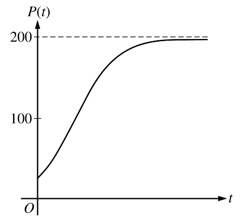
\includegraphics[scale=0.9]{original-6.png}
    \end{center}
    Which of the following differential equations for a population P could model the logistic growth shown in the figure above?
    $$\lim_{t\to\infty} P(t) = 200$$
    $$\boxed{\frac{dP}{dt}=0.2P-0.001P^2}$$
\end{enumerate}
\end{document}
